\chapter{ارزیابی و نتایج}
\label{chap:evaluation}

در این فصل چارچوب بر معیارهای عملی ارزیابی می‌شود: پوشش سناریوها، نتیجه‌ی اجرای کامل، گزارش‌گیری و مسیر انتقال به پایپلاین‌ی
\lr{\gls{CI}}/\lr{\gls{CD}}.

\section{محیط آزمایش}
همه‌ی ارزیابی روی یک سامانه‌ی ویندوزی واقعی انجام شده است؛ مشخصات محیط به پیروی از رویه‌ی گزارش‌های مهندسی، فهرست‌وار آورده می‌شود:
\begin{itemize}
	\item سیستم‌عامل: ویندوز ۱۱ (میزکار) با فعال‌بودن حالت توسعه‌دهنده
	\item زبان و کیت برنامه‌ی نمونه:
	\lr{Qt 6.8.3 (MinGW 13.1), CMake, Ninja}
	\item زبان چارچوب:
	\lr{Python 3.12}
	با
	\lr{pytest}
	و
	\lr{Appium Python Client}
	\item سرور درایور:
	\lr{Appium 3}
	روی درگاه ۴۷۲۳ و
	\lr{WinAppDriver}
	برای مسیر اجرای بی‌سر
	\gls{HeadlessRun}
	\item گزارش‌ساز:
	\lr{Allure 3}
	\item سخت‌افزار: رایانه‌ی شخصی با پردازنده‌ی
	\lr{x86\_64}
	و ۱۶ گیگابایت حافظه
\end{itemize}

\section{سوییت سناریوها}
۲۵ سناریوی سرتاسری نوشته شده که به شش خانواده تقسیم می‌شوند: جریان ورود و ثبت‌نام (۵ سناریو)، فیلترهای جدول شبکه (۶ سناریو)، صفحه‌بندی و شناسه‌ی ردیف‌ها (۳ سناریو)، داشبورد (۴ سناریو شامل سنجش نمودار دایره‌ای و ستونی در برابر داده‌ی مستخرج از خروجی
\lr{\gls{CSV}})،
گزارش‌ها (۴ سناریو شامل انتقال فیلتر و گروه‌بندی) و تست‌های زیرساخت (۲ سناریو). در کنار این‌ها، دو تست داخلی برنامه (تست دود رابط کاربری و تست لایه‌ی داده) و یک سناریوی نمایشی عمداً شکست‌خورده وجود دارد که نقش آن، نشان‌دادن رفتار گزارش‌گیری در هنگام خطا در جلسه‌ی نمایش است.

نکته‌ی مهم در سناریوهای نمودار این است که تست، خروجی
\lr{\gls{CSV}}
همان فیلتر را از زبانه‌ی شبکه استخراج و توزیع داده را مستقل از برنامه محاسبه می‌کند؛ سپس برش‌های خوانده‌شده از فهرست آینه‌ی نمودار را با آن مقایسه می‌کند. به این ترتیب درستیِ نمودار با «منبع حقیقت دیگری» سنجیده می‌شود نه با خود برنامه.

\section{اجرای کامل و گزارش}
اجرای کامل مجموعه در حدود شش دقیقه انجام می‌شود؛ خروجی پایدار آن ۲۴ سناریوی موفق و یک شکست عمدی است. گزارش
\lr{Allure}
این اجرا در شکل
\autoref{fig:allure}
نمایش داده شده است: شمار کل، موفق و شکست به تفکیک فایل سناریو، با زمان‌بندی هر تست. در صورت شکست هر تست، تصویر لحظه‌ی خطا به گزارش پیوست می‌شود.

\begin{figure}[H]
\centering
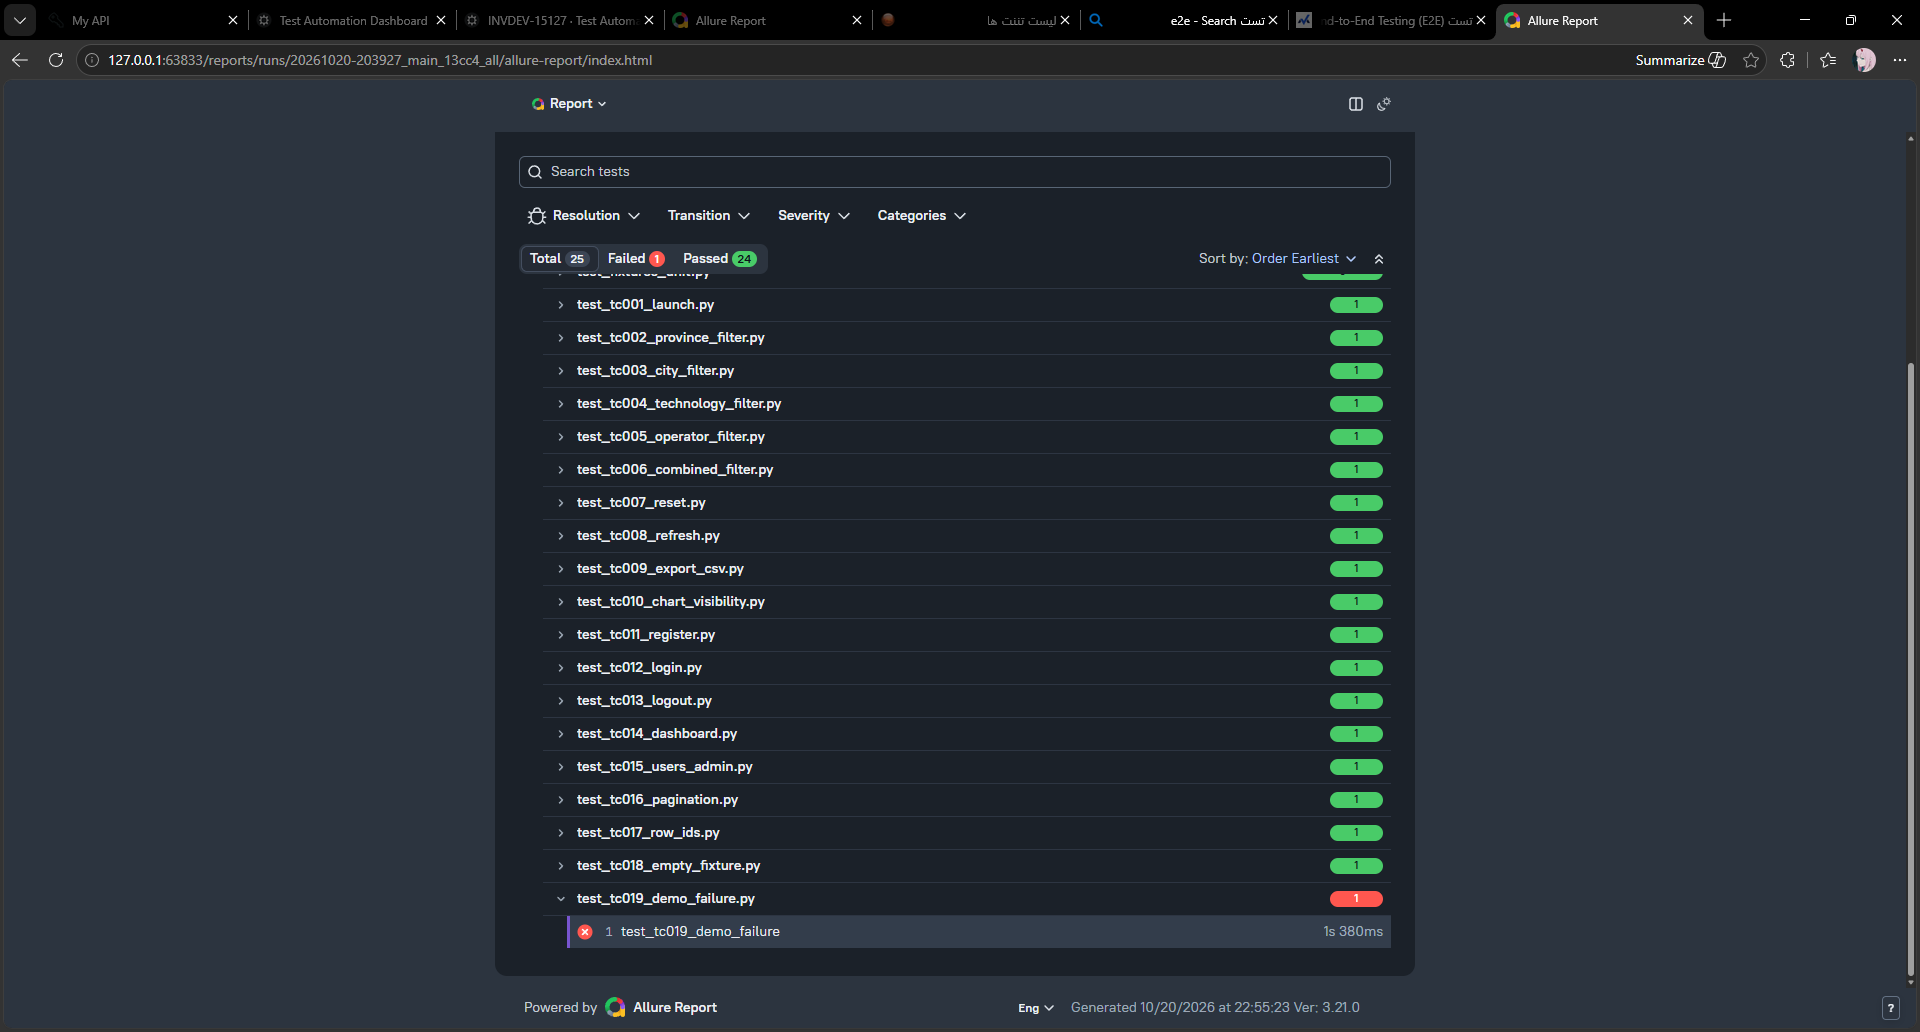
\includegraphics[width=\linewidth]{fig_allure}
\caption{گزارش \lr{Allure} پس از اجرای کامل مجموعه؛ شکست عمدی سناریوی نمایشی آشکار است}
\label{fig:allure}
\end{figure}

برای نشان‌دادن جریان کامل اجرا، یک فیلم کوتاه از اجرای کل مجموعه ضبط شده است. در نسخه‌ی الکترونیکی این پایان‌نامه، ویدیوی زیر با کلیک فعال می‌شود:

\begin{figure}[H]
\centering
\includemedia[
	width=0.9\linewidth,
	height=0.51\linewidth,
	activate=pagevisible,
	addresource=fig_suite_run.mp4,
	flashvars={source=fig_suite_run.mp4&autoPlay=false&loop=true}
]{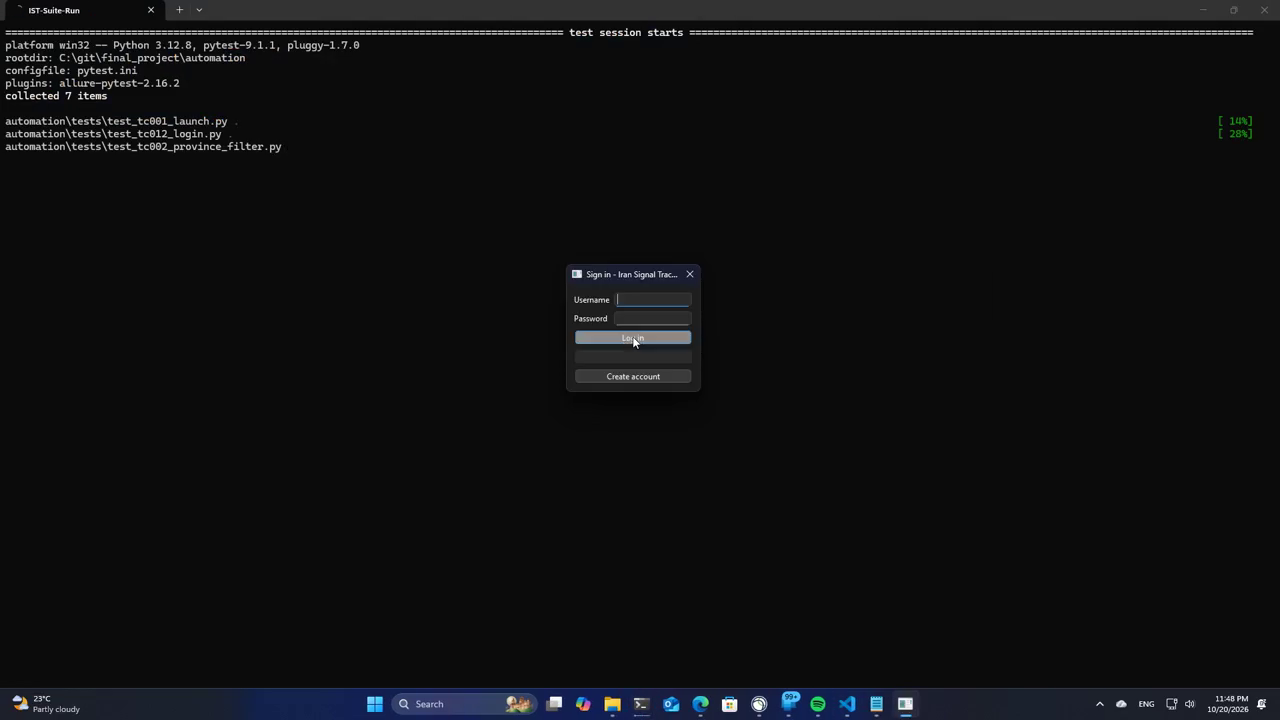
\includegraphics[width=0.9\linewidth]{fig_suite_poster}}{VPlayer.swf}
\caption{فیلم اجرای کامل سوییت سرتاسری (نیازمند نمایشگر \lr{PDF} تعاملی)}
\label{fig:video}
\end{figure}

در نسخه‌ی چاپی، شکل‌های
\autoref{fig:signin}
تا
\autoref{fig:allure}
در فصل‌های قبلی جریان را بازگو می‌کنند.

\section{انتقال به پایپلاین \lr{CI/CD}}
چارچوب از ابتدا برای سوار‌شدن بر پایپلاین طراحی شده است. شکل هدف پایپلاین چنین است:
\begin{latin}
\begin{lstlisting}[language=bash, numbers=none]
Commit
  -> Build App        (cmake configure + build; ctest smoke + db_test gate)
  -> Launch Appium    (appium server on :4723)
  -> Launch Application (driver factory starts the exe via caps)
  -> Execute Tests    (python -m pytest automation/tests)
  -> Generate Allure  (allure generate ... -o reports/allure-report)
  -> Publish Report   (host allure-report artefact, if: always())
\end{lstlisting}
\end{latin}

نکات طراحی‌شده برای نویسنده‌ی پایپلاین: نهان‌گاه کردن مسیرهای
\lr{Qt}
،
\lr{MinGW}
و
\lr{Python}
بر اساس پین‌های نسخه در مستندات محیط؛ نیاز رانر به ویندوز، حالت توسعه‌دهنده و نصب
\lr{WinAppDriver}؛
شکست هر تست به معنی شکست کار بدون حذف انتشار گزارش (با شرط
\lr{always()})
؛ و مسیر اجرای بی‌سر با
\lr{DRIVER\_MODE=direct}
که سرور
\lr{Appium}
را از معادله حذف می‌کند و مستقیماً به
\lr{WinAppDriver}
وصل می‌شود. جداسازی پایگاه‌داده در سطح تست (فصل
\autoref{chap:framework})
ضمانت می‌کند که اجراهای موازی‌نما و متوالی روی یک رانر، به هم آلودگی ایجاد نکنند.

\section{تحلیل نتایج}
سه شاهد کیفی از ارزیابی قابل استناد است. نخست، پایداری: کل مجموعه در چندین اجرای پیاپی با همان نتیجه اجرا شده و تنها شکست‌ها، شکست عمدی سناریوی نمایشی بوده است. دوم، سرعت: با بخش‌بندی درخت مکان‌یابی و نهانگاه دسته‌ها، زمان اجرای کامل از حدی که عملاً غیرقابل‌استفاده بود (جستجوهای تک‌ثانیه‌ای تا ۱۱ ثانیه) به حدود شش دقیقه برای ۲۵ سناریو رسید. سوم، نگهداشت‌پذیری: در طول توسعه، تغییرات متعددی در چیدمان رابط کاربری برنامه (جابه‌جایی پنل‌ها، افزودن نمودار) رخ داد که هیچ‌یک تستی را نشکست؛ تنها لایه‌ی اشیای صفحه تغییر کرد — همان چیزی که جداسازی لایه‌ها وعده می‌داد. محدودیت‌های چارچوب نیز روشن است: وابستگی به ویندوز و
\lr{WinAppDriver}،
نیاز برنامه‌های هدف به رعایت قراردادهای پایداری، و اجرای تعاملی (نه هم‌زمان) برای درایورهای پنجره‌ای.